\section{Proposed Method}
\label{sec:propwork-atpo-method}

\begin{figure*}
	\centering
	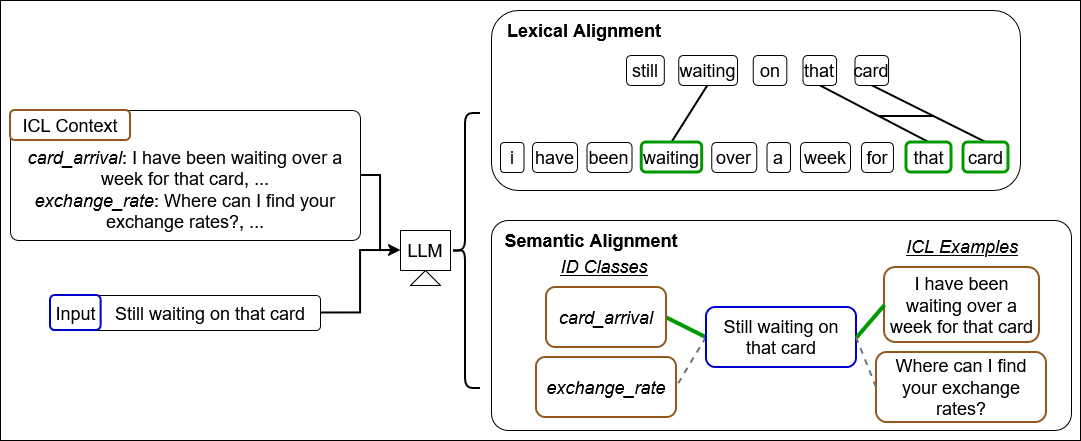
\includegraphics[width=1.\linewidth]{figures/align_examples}
	
	\caption{Examples of lexical and semantic alignment induced in an LLM via ICL prompting. Orange represents the ICL context, blue represents the input, and green represents strong alignment. The input is strongly aligned with the ``card\_arrival'' category and examples but not strongly aligned with the ``exchange\_rate'' cateory and examples. 
	}
	\label{fig:atpo_alignexamples}
\end{figure*}

%The proposed \sys leverages the latent knowledge in LLMs for OOD detection using only text prompts. It solves the prompt-only OOD detection problem by first extracting fine-grained knowledge through \textit{alignment} of the input text with ID classes (category labels) and few-shot examples for those classes provided in the \textit{in-context learning (ICL)} prompt. Second, \sys uses the alignment reasoning to generate a continuous OOD score for a sample. The OOD scores for the ID data are used to calculate a \textit{threshold} for OOD detection instead of performing ($C$+1)-classification.
In \gls{syst}, prompt-only OOD detection is performed by leveraging the latent knowledge in LLMs via text prompts. First, fine-grained knowledge is extracted through \textit{alignment} between the input test utterance and ID classes (i.e. the category labels for included ID classes in each dataset) and associated few-shot examples for each class. This \textit{ICL information} and the test utterance are then used, contextualized by the alignment reasoning, to generate an OOD score for the input. This continuous score is generated for all ID test data which is finally used to calculate a \textit{threshold} for OOD detection.

\subsection{Prompt Context and Alignment}

%%\vspace{2mm}
%%\noindent
%\paragraph{In-Context Learning.} Contextualization of any given input $x$ is provided through few-shot ICL. 
%We randomly select $m$ demonstration examples from each ID class to create a demonstration set as context $\mathcal{C}$. Specifically, using ID training examples and labels $(t_i,y_i)$, we curate $\mathcal{C} = \bigcup_{j=1}^{C} \{(t_i,y_i) | y_i = j\}_{i=1}^{m}$ and provide it to an LLM along with the input. Results across the number of ICL examples $m$ and number of ID classes $C$ are presented in Section \ref{sec:disc}.
\subsubsection{In-Context Learning}
For any given input test utterance $x$, contextualization is formulated as few-shot ICL.
A context $\mathcal{C}$ demonstration set is created by randomly selecting $\nu$ demonstration examples from each ID class. Specifically, ID training examples and labels $(t_i,y_i)$ are used to curate context $\mathcal{C} = \bigcup_{j=1}^{C} \{(t_i,y_i)\ |\ y_i = j\}_{i=1}^{\nu}$ for number of ID classes $C$. The context $\mathcal{C}$ is provided to the LLM along with the input test utterance in a prompt $P$.

% li2025tokalign (align = cosine sim)
% https://d197for5662m48.cloudfront.net/documents/publicationstatus/231698/preprint_pdf/889ad760a1b1d9b655bcee61da7b1ac2.pdf - for some potential math
% el2021xlent (lexical and semantic align defs)
% dyer2013simple (fastalign, word align) - for math
% thompson2020cultural (semantic align - meaning of words/phrases are similar)
% srivastava2025measuring (lexical align review) - for some potential math

%%\noindent
\subsubsection{Alignment} 

%We consider here the alignment between an input $x$ and the ID classes $\mathcal{Y}_{ID} = \{1,2,\dots,C\}$ and examples $\mathcal{C}_t = \bigcup_{j=1}^{C} \{t_i | y_i = j\}_{i=1}^{m}$. Specifically, ``alignment'' in this work refers to the \textit{similarity} between the input and the ID classes and their examples in an established comparison space. In the case of ``lexical alignment'', this similarity space is characterized by the \textit{words} in the input and context. In the case of ``semantic alignment'', this similarity space is characterized by the \textit{meaning} associated with the words and phrases in (or the entirety of) the input and context. Note that we do \textit{not} consider Human-LLM alignment \citep{wang2023aligning, ji2023ai} here which is a different topic.
%
%The LLM $f_{LLM}$ establishes the lexical and semantic similarity spaces in which alignment can be performed using the ID classes $\mathcal{Y}_{ID}$ and ICL examples $\mathcal{C}_t$.
%By using the knowledge and reasoning capabilities inherent to LLMs \citep{kumar2025llm}, the LLM identifies the components defining the similarity spaces in the input $x$ and context $\mathcal{C}$. These spaces enable the measurement of alignment between $x$ and the ID classes $\mathcal{Y}_{ID}$ and ICL examples $\mathcal{C}_t$. 
%
%In previous alignment work, the components defining the lexical and semantic spaces would be defined by the user (e.g., cosine similarity) \citep{dyer2013simple,srivastava2025measuring}. However, as we are limited to only prompts, the lexical and semantic spaces and subsequent alignment must be generated entirely by the LLM through the prompt $\mathcal{P}$. 
%
%We induce lexical and semantic alignment in $f_{LLM}$ between $x$ and $(\mathcal{Y}_{ID},\mathcal{C})$ through the prompted generation of \textit{alignment scores} $\mathcal{A} \sim f_{LLM}(\mathcal{P}(x|\mathcal{Y}_{ID},\mathcal{C}))$ where
%\begin{equation}
%\begin{aligned}
%    \mathcal{A}_1 & \sim f_{LLM}(\mathcal{P}(x|y_1,\mathcal{C}_{t,1})) \\
%    \mathcal{A}_2 & \sim f_{LLM}(\mathcal{P}(x|y_2,\mathcal{C}_{t,2})) \\
%    \dots \\
%    \mathcal{A}_C & \sim f_{LLM}(\mathcal{P}(x|y_C,\mathcal{C}_{t,C})), \\
%\end{aligned}
%\end{equation}
%where $\mathcal{A}_i \in \mathbb{R}$ is the alignment score between $x$ and the class $y_i$ with ICL examples $\mathcal{C}_{t,i} = \{t_k | y_k = i\}_{k=1}^{m}$. $\mathcal{A}$ represents the similarity between $x$ and the ID distribution defined by the lexical and semantic spaces informed by the LLM's knowledge and provided context. These alignment scores subsequently inform OOD detection.
Alignment is defined in this study between an input $x$ and ID classes $\mathcal{Y}_{ID} = \{1,2,\dots,C\}$ and ICL examples $\mathcal{C}_t = \bigcup_{j=1}^{C} \{t_i\ |\ y_i = j\}_{i=1}^{\nu}$. The specific ``alignment'' considered is the \textbf{similarity} between the input and the ID classes and ICL examples in some comparison space. Two comparison spaces are established for this work. First, ``lexical alignment'', is a comparison space characterized by the \textit{words} in the input and the context, i.e. the words comprising the ID classes and in the ICL examples. Second, ``semantic alignment'', is a comparison space characterized by the \textit{meaning} associated with the words and phrases in (or entirety of) the input, the ID classes, and the ICL examples. Semantic alignment measures similarities between the meanings within the input and the meanings present in the context. An example of both types of alignment is shown in \ref{fig:atpo_alignexamples}. Importantly, ``alignment'' here does not refer to Human-LLM alignment \cite{wang2023aligning,ji2023ai} which is an entirely different topic and is not relevant.

An LLM $f_{LLM}$ establishes the lexical and semantic comparison spaces for alignment using the ID classes $\mathcal{Y}_{ID}$ and ICL examples $\mathcal{C}_t$. Through the knowledge and reasoning capabilities inherent to LLMs \cite{kumar2025llm}, the LLM can isolate and extract components in the input $x$ and context $\mathcal{C}$ that define the comparison spaces. These spaces define the measurement basis of alignment between $x$ and the ID classes $\mathcal{Y}_{ID}$ and ICL examples $\mathcal{C}_t$. In previous works on alignment, lexical and semantic spaces would be defined by the user (e.g. cosine similarity) \cite{dyer2013simple,srivastava2025measuring}. Given that prompt-only OOD detection methods are limited to prompts, these definitions are not possible. Instead, the lexical and semantic spaces (as well as subsequent alignment) must be generated entirely through the LLM via prompt $P = \mathcal{P}(\cdot)$ for prompt template $\mathcal{P}$ (see Section \ref{sec:atpo_pinfo} for details). In \gls{syst}, lexical and semantic alignment is induced in $f_{LLM}$ between $x$ and $(\mathcal{Y}_{ID},\mathcal{C})$ through the generation of \textit{alignment scores} $\mathcal{Q} \sim f_{LLM}(\mathcal{P}(x\ |\ \mathcal{Y}_{ID},\mathcal{C}))$ where
\begin{equation}
\begin{aligned}
    \mathcal{Q}_1 & \sim f_{LLM}(\mathcal{P}(x\ |\ y_1,\mathcal{C}_{t,1})) \\
    \mathcal{Q}_2 & \sim f_{LLM}(\mathcal{P}(x\ |\ y_2,\mathcal{C}_{t,2})) \\
    \dots \\
    \mathcal{Q}_C & \sim f_{LLM}(\mathcal{P}(x\ |\ y_C,\mathcal{C}_{t,C})), \\
\end{aligned}
\end{equation}
where any $\mathcal{Q}_i \in \mathbb{R}$ is the alignment score between input test utterance $x$ and the class $y_i$ at $i$. Additionally, $\mathcal{C}_{t,i} = \{t_k\ |\ y_k = i\}_{k=1}^{\nu}$ is the associated ICL examples for class $y_i$.

\subsection{OOD Detection via Thresholding}

%%\vspace{2mm}
%%\noindent
%%\textbf{OOD Scoring.} 
%A function $\mathsf{Parse}(\cdot)$ is used to extract the OOD score $s$ from the generated output of an LLM model $f_{LLM}$
%\begin{equation}
%\begin{split}
%	s & = \mathsf{Parse}(f_{LLM}(\mathcal{P}(x|\mathcal{Y}_{ID},\mathcal{C}))). \\
%\end{split}
%\end{equation}
%The LLM $f_{LLM}$ implicitly utilizes the alignment scores $\mathcal{A}$ during generation to weigh the lexical and semantic similarity between the input $x$ and the ID context $\mathcal{C}$. The alignment informs the extraction of OOD score $s$ by reasoning across the ID classes and ICL examples, as demonstrated in the preceding qualitative study.
%Example outputs $f_{LLM}(\mathcal{P}(x|\mathcal{Y}_{ID},\mathcal{C}))$ are in Section \ref{sec:disc}.
%
%OOD detection is performed by applying a threshold $t_{ID}$ to OOD scores $s$
%\begin{equation}
%  S(s, t_{ID}) =
%  \begin{cases}
%    \text{ID,} & \text{$s \geq t_{ID}$} \\
%    \text{OOD,} & \text{$s < t_{ID}$}. \\
%  \end{cases}
%\end{equation}
%OOD detection performance can be formulated as multiple thresholds over ranked OOD scores (Area Under the Receiver Operating Characteristic curve, AUC) or as a single threshold informed by the statistics of the ID data distribution (95\% False Positive Rate, FPR95) \citep{zhang2023openood}. By leveraging the OOD scores for ID data, OOD detection can be improved through the informed separation of the ID score space and the OOD score space. In particular, near-OOD samples are better detected in this paradigm because uncertain ID samples (which may be similar to near-OOD samples) are considered for the threshold calculation. This is impossible for the previous prompt-only OOD detection method \citep{wang2024beyond} because their direct ($C$+1)-class decision approach \textit{has no notion of OOD scoring}.
%\paragraph{Generation Parsing.} We parse generated outputs to ensure consistency and valid generation of intents and ``unknown''. To prevent false positives from LLM generation of multiple intents or classes (perhaps seen from in-context learning examples), we discard any generated responses containing more than one intent as invalid. Furthermore, to allow for minor variation in generated response, we allow generation up to 7 tokens and check if the number of matched intent tokens is the majority of generated tokens. This handles cases where the ground truth intent is ``card\_payment\_wrong\_exchange\_rate'' but the generated response may be ``incorrect exchange rate for the card payment''.
A function $\mathsf{Parse}(\cdot)$ is used to extract the OOD score $s$ from the generated output of an LLM model $f_{LLM}$
\begin{equation}
\begin{split}
	s & = \mathsf{Parse}(f_{LLM}(\mathcal{P}(x\ |\ \mathcal{Y}_{ID},\mathcal{C}))). \\
\end{split}
\end{equation}
for prompt template $\mathcal{P}$. Specifically, generated outputs are split on a key-phrase ``OOD Score:'' (which was instructed for in the prompt). The most recently generated valid float value generated after the key-phrase was considered as the OOD score.

The alignment scores $\mathcal{Q}$ are used implicitly by $f_{LLM}$ during generation. They assist in quantifying and weighing the lexical and semantic similarity between the input test utterance $x$ and the context $\mathcal{C}$ containing the ID classes and ICL examples. This alignment procedure informs extraction of the OOD score $s$ via reasoning across the ID information.

OOD detection is subsequently performed using OOD scores $s$ by applying a threshold $h_{ID}$
\begin{equation}
  S(s, h_{ID}) =
  \begin{cases}
    \text{ID,} & \text{$s \geq h_{ID}$} \\
    \text{OOD,} & \text{$s < h_{ID}$}. \\
  \end{cases}
\end{equation}
As previously defined in Chapter \ref{diss_bkgd}, metrics for OOD detection rely on some characterization of a threshold and evaluation of the test ID and OOD data against this threshold. To reiterate in the context of prompt-only OOD detection and \gls{syst}, the Area Under the Receiver Operating Characteristic curve (AUC) is an OOD detection metric that uses multiple thresholds over ranked OOD scores. Another OOD detection metric, True Positive Rate at 95\% False Positive Rate (FPR95), uses a single threshold informed by the statistics of the ID data distribution. Leveraging OOD scores for test ID data enables OOD detection through the informed distinction of the ID and OOD score spaces. In particular, and most relevant for this dissertation, near-OOD samples are more effectively detected using ID-informed thresholds because uncertain ID samples (which are very similar to near-OOD samples) are \textit{accounted for in the threshold calculation}. This is impossible for the previous prompt-only OOD detection method \cite{wang2024beyond}. In ($C$+1)-classification, there is \textit{no functionality for OOD scoring}. Thus the ID data distribution cannot be considered during OOD detection.
%$s$ is used for OOD detection of the input $x$ in two ways. First, the continuous range of scores $s \in [0,1]$ allows for a larger metric space for OOD detection compared to the binary decision method proposed in \citet{wang2024beyond}. This establishes OOD detection by considering thresholds across the range of $s$, analogous to the widely-accepted Area Under the Receiver Operating Characteristic curve (AUC) established in OOD detection literature \cite{zhang2023openood}. $s$ may also be used via selecting a single threshold $t_{ID}$
%\begin{equation}
%  S(s, t_{ID}) =
%  \begin{cases}
%    \text{ID,} & \text{$s \geq t_{ID}$} \\
%    \text{OOD,} & \text{$s < t_{ID}$} \\
%  \end{cases}
%\end{equation}
%Both of these approaches are based on the ranking of scores $s$ output from the LLM from ICL and lexical and semantic alignment. They improve upon the previous prompt-only OOD detection method \cite{wang2024beyond}, which used a binary decision for each input $x$, by \textit{quantifying the degree of alignment}. The approach proposed by \citet{wang2024beyond} struggles with detecting samples near the decision boundary as the uncertainty of such ambiguous samples is not accounted for in the detection process. In \sys, the low alignment of such a sample is considered in the detection and provides a clear OOD score metric that establishes \textbf{how much} the input is OOD. This allows subsequent thresholding, whether through AUC or 95\% False Positive Rate \cite{zhang2023openood}, to account for a greater range of possible OOD samples instead of relying only on binary ID and OOD classes.

\subsection{Prompt Instantiation}
\label{sec:atpo_pinfo}

%%\vspace{2mm}
%%\noindent
%%\textbf{Prompt Instantiation.} 
%The ID classes $\mathcal{Y}_{ID}$, ICL context $\mathcal{C}$, and input $x$ are used to instantiate the prompt $P$ from prompt template $\mathcal{P}$, $P = \mathcal{P}(x|\mathcal{Y}_{ID},\mathcal{C})$. Our prompt template $\mathcal{P}$ differs from that of \citet{wang2024beyond} in two ways: 1) we directly encourage alignment between $x$ and ICL context $\mathcal{C}$ for OOD detection, and 2) we do not require the LLM to classify $x$, only provide an OOD score. We share $\mathcal{P}$ and examples in Appendix Section 4.
The prompt $P$ for \gls{syst} is instantiated with ID classes $\mathcal{Y}_{ID}$, ICL context $\mathcal{C}$, and input $x$ through a prompt template $\mathcal{P}$, $P = \mathcal{P}(x\ |\ \mathcal{Y}_{ID},\mathcal{C})$. Crucially, the prompt template proposed in \gls{syst} differs from the previous baseline in that 1) alignment between $x$ and context $\mathcal{C}$ is directly encouraged through lexical and semantic spaces, and 2) LLMs are not required to classify $x$, only provide an OOD score.

\subsection{Prompts}
\label{sec:app-prompts}

The prompt templates used by \gls{syst} are detailed here along with examples. For illustrative purposes, all examples are included with only 1 ICL example per class.

The \gls{syst} template is:
\begin{quote}
You are a language model-based Out-of-Distribution (OOD) detector. Your task is to use your internal reasoning to estimate an OOD score for a given test utterance given some contextual In-Distribution (ID) categories and example utterances.

Here are definitions that will elucidate the concepts relevant to your task:

- ID: The samples, i.e. utterances and categories, that define the data domain you are responsible for. You should be familiar with these categories and are trying to identify if any given test utterance is within the ID categories (using the category topics and ID example utterances to help your decision).

- OOD: Everything that is NOT within the ID data domain. Any sample that does not fall within or align with the ID categories and utterances is OOD.

- Lexical alignment: The concept of similarity between a test utterance and the ID data domain based on LEXICAL factors. This includes similarity concepts such as keyword matching, phrasing similarity, and grammatical/tuple patterns.

- Semantic alignment: The concept of similarity between a test utterance and the ID data domain based on SEMANTIC factors. This includes similarity concepts such as closeness of meanings or themes, conceptual comparisons, and similarity of the presented ideas.

1. Category Matching: For each ID category, estimate how well the utterance aligns with it and its examples. Rank the degree of alignment considering the lexical alignment and semantic alignment.

2. Confidence Estimation: Based on your ranking, assign an OOD score indicating how well the top-ranked category aligns with the test utterance. If the utterance does not align well with the top-ranked category, assign a high OOD score. If it aligns strongly with the top-ranked category, assign a low OOD score.

Now apply these steps to the following input:

In-Distribution categories: \{\}

Example In-Distribution utterances:

\{\}

Test utterance: \{\}

Respond with the following information:

Reasoning: <text with your reasoning> 

OOD Score: <float from 0.0 (confidently in-distribution) to 1.0 (confidently out-of-distribution)>

Response:
\end{quote}
An example is:
\begin{quote}
You are a language model-based Out-of-Distribution (OOD) detector. Your task is to use your internal reasoning to estimate an OOD score for a given test utterance given some contextual In-Distribution (ID) categories and example utterances.

Here are definitions that will elucidate the concepts relevant to your task:

- ID: The samples, i.e. utterances and categories, that define the data domain you are responsible for. You should be familiar with these categories and are trying to identify if any given test utterance is within the ID categories (using the category topics and ID example utterances to help your decision).

- OOD: Everything that is NOT within the ID data domain. Any sample that does not fall within or align with the ID categories and utterances is OOD.

- Lexical alignment: The concept of similarity between a test utterance and the ID data domain based on LEXICAL factors. This includes similarity concepts such as keyword matching, phrasing similarity, and grammatical/tuple patterns.

- Semantic alignment: The concept of similarity between a test utterance and the ID data domain based on SEMANTIC factors. This includes similarity concepts such as closeness of meanings or themes, conceptual comparisons, and similarity of the presented ideas.

1. Category Matching: For each ID category, estimate how well the utterance aligns with it and its examples. Rank the degree of alignment considering the lexical alignment and semantic alignment.

2. Confidence Estimation: Based on your ranking, assign an OOD score indicating how well the top-ranked category aligns with the test utterance. If the utterance does not align well with the top-ranked category, assign a high OOD score. If it aligns strongly with the top-ranked category, assign a low OOD score.

Now apply these steps to the following input:

In-Distribution categories: \textit{card\_arrival, card\_linking, exchange\_rate, card\_payment\_wrong\_exchange\_rate, extra\_charge\_on\_statement}

Example In-Distribution utterances:

\textit{card\_arrival: [Is there a way to track the delivery of my card?], ...}

   \textit{card\_linking: [How do I add an existing card to the app?], ...}
   
   \textit{exchange\_rate: [Where can I find your exchange rates?], ...}
   
   \textit{card\_payment\_wrong\_exchange\_rate: [The exchange rate was incorrect for an item I bought.], ...}
   
   \textit{extra\_charge\_on\_statement: [I have been charged a pound for something that appears on my statement], ...}
   
Test utterance: \textit{How do I locate my card?}

Respond with the following information:

Reasoning: <text with your reasoning> 

OOD Score: <float from 0.0 (confidently in-distribution) to 1.0 (confidently out-of-distribution)>

Response:
\end{quote}

The prompt for \gls{syst} can be modulated in several ways to account for various degrees of induced alignment. In one modulation, denoted as Nonspecified Alignment, alignment is still induced but it is not specified to the LLM that lexical and semantic alignment should be considered.
For \gls{syst}-Nonspecified Alignment, the template is:
\begin{quote}
You are a language model-based Out-of-Distribution (OOD) detector. Your task is to use your internal reasoning to estimate an OOD score for a given test utterance. You will also be provided with the set of In-Distribution (ID) categories and several example utterances from each category as additional context. Use the following structured reasoning steps to estimate an OOD score for a given test utterance:

1. Category Matching: For each ID category, estimate how well the utterance aligns with it and its examples. Use your knowledge of language, context, and category semantics, along with the examples for each category, to rank the degree of alignment.

2. Confidence Estimation: Based on your ranking, assign an OOD score indicating how well the top-ranked category aligns with the test utterance. If the utterance does not align well with the top-ranked category, assign a high OOD score. If it aligns strongly with the top-ranked category, assign a low OOD score.

Now apply these steps to the following input:

In-Distribution categories: \{\}

Example In-Distribution utterances:

\{\}

Test utterance: \{\}

Return an OOD score from 0.0 (confidently in-distribution) to 1.0 (confidently out-of-distribution).

Response:
\end{quote}
Similarly, for \gls{syst} with only reasoning and no specified lexical or semantic alignment (denoted as ``Reasoning''), modulated behavior is induced that continues to leverage alignment-based reasoning over the ID classes and ICL context but not to the depth proposed in \gls{syst}.
For \gls{syst}-Reasoning, the template is:
\begin{quote}
You are a language model-based Out-of-Distribution (OOD) detector. Your task is to use your internal reasoning to estimate an OOD score for a given test utterance. You will also be provided with the set of In-Distribution (ID) categories and several example utterances from each category as additional context. Use the following structured reasoning steps to estimate an OOD score for a given test utterance:

1. Category Matching: For each ID category, estimate how well the utterance aligns with it and its examples. Use your knowledge of language, context, and category semantics, along with the examples for each category, to rank the degree of alignment.

2. Confidence Estimation: Based on your ranking, assign an OOD score indicating how well the top-ranked category aligns with the test utterance. If the utterance does not align well with the top-ranked category, assign a high OOD score. If it aligns strongly with the top-ranked category, assign a low OOD score.

Now apply these steps to the following input:

In-Distribution categories: \{\}

Example In-Distribution utterances:

\{\}

Test utterance: \{\}

Respond with the following information:

Reasoning: <text with your reasoning>

OOD Score: <float from 0.0 (confidently in-distribution) to 1.0 (confidently out-of-distribution)>

Response:
\end{quote}
